\documentclass[12pt,a4paper]{article}

\newcommand{\diff}[1]{d#1}
\newcommand{\dd}[2]{\frac{\partial #1}{\partial #2}}

\usepackage{amsmath}
\usepackage{graphicx}
\usepackage{float}
%---------------------------------------------------------------------------
\begin{document}
%---------------------------------------------------------------------------	
	
\section{Objetivo}

O objetivo final deste texto é chegar a um modelo de uma equação de um problema elástico não-linear unidimensional. Para isso a equação de equilíbrio estático será discretizado via elementos finitos. A malha será constituída de apenas um elemento linear. O problema considerado será semi-estático devido ao passo de carregamento. O tempo sera considerado de maneira discreta através de $t_n = n$ e $t_{n+1} = n+1$

A Figura \ref{fig:problema} apresenta o problema resolvido. A barra esta engastada de parede à esquerda e um força é aplicada a direita. A geometria da barra é definida pelo comprimento $L$ e área transversal "A". Para simplifica será considerada uma área unitária.

\begin{figure}[H]
	\centering
	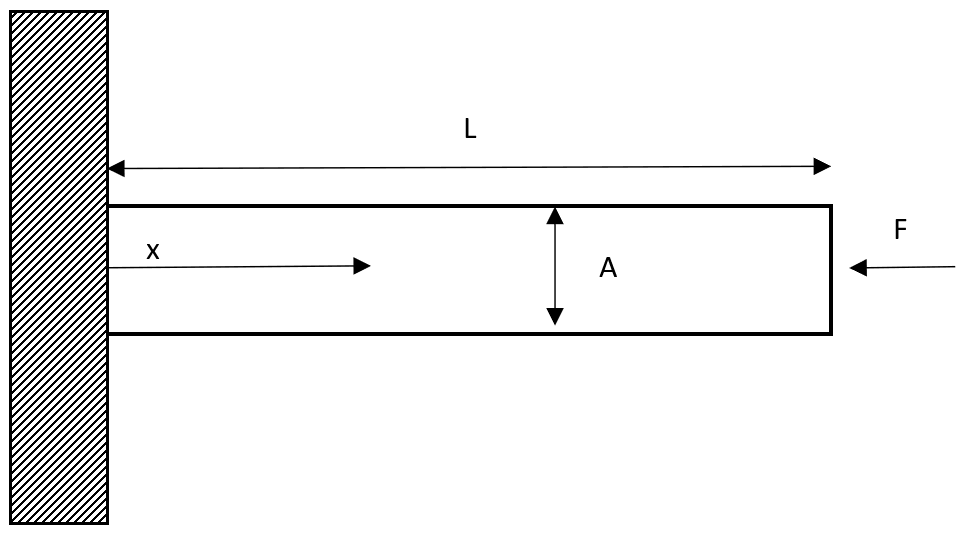
\includegraphics[width=0.6\textwidth]{problema.PNG}
	\caption{Problema um 1D de elasticidade.}
	\label{fig:problema}
\end{figure}

\subsection{Equação de elasticidade 1D}

A equação de elasticidade 1D sem forças de corpo é dada por,

\begin{equation}
	\dd{\sigma}{x} = 0
	\label{eq_equilibrio}
\end{equation}
	
\noindent
onde $\sigma$ é a tensão uniaxial.

\subsection{Discretização via elementos finitos}

Aplicando o método dos resíduos ponderados na (eq.\ref{eq_equilibrio}) tem-se,

\begin{equation}
\int_0^L{\dd{\sigma}{x}w\diff{L}} = 0
\label{eq_residuos_pon}
\end{equation} 

Considerando a regra do produto para derivadas temos,

\begin{equation}
\dd{(\sigma w)}{x} = \dd{\sigma}{x}w + \dd{w}{x}\sigma
\end{equation} 
 
E considerando que que,

\begin{equation}
\int_0^L \dd{(\sigma w)}{x} \diff{L} = \sigma w |_0^L
\end{equation} 
 
Logo pode-se escrever a (eq.\ref{eq_residuos_pon}) como,

\begin{equation}
\int_0^L \dd{w}{x}\sigma \diff{L} = \sigma w |_0^L
\label{eq_var}
\end{equation}

Considerando apenas um elementos a função de ponderação é dada por,

\begin{equation}
w(x) = N_1(x) w_1 + N_2(x) w_2
\end{equation} 
	
Substituindo a função $w$ na equação (eq.\ref{eq_var}),

\begin{equation}
\begin{split}
&\int_0^L \left( \dd{N_1}{x}w_1 + \dd{N_2}{x}w_2 \right)\sigma \diff{L} =\\
&\left(N_1(L) w_1 + N_2(L) w_2\right) \sigma\left(L,t\right) - \left(N_1(0) w_1 + N_2(0) w_2\right) \sigma\left(0,t\right)
\end{split}
\end{equation}
	
Rearranjando os termos temos,

\begin{equation}
\begin{split}
&w_1\left( \int_0^L \dd{N_1}{x}\sigma \diff{L} - N_1(L) \sigma\left(L,t\right) + N_1(0) \sigma\left(0,t\right) \right) +\\
&w_2\left( \int_0^L \dd{N_2}{x}\sigma \diff{L} - N_2(L) \sigma\left(L,t\right) + N_2(0) \sigma\left(0,t\right) \right) = 0
\end{split}
\end{equation}

Considerando que $N_1(0) = N_2(L) = 1$ e $N_1(L) = N_2(0) = 0$,

\begin{equation}
\begin{split}
w_1\left( \int_0^L \dd{N_1}{x}\sigma \diff{L} + \sigma\left(0, t\right) \right) +
w_2\left( \int_0^L \dd{N_2}{x}\sigma \diff{L} - \sigma\left(L, t\right) \right) = 0
\end{split}
\end{equation}
	
Como $w_1$ e $w_2$ são constantes arbitrarias é preciso que,

\begin{equation}
\int_0^L \dd{N_1}{x}\sigma \diff{L} + \sigma\left(0, t\right) = 0
\label{eq_u1}
\end{equation}

\begin{equation}
\int_0^L \dd{N_2}{x}\sigma \diff{L} - \sigma\left(L, t\right) = 0
\label{eq_u2}
\end{equation}
 
Definindo $B_i = \dd{N_i}{x}$, tem-se

\begin{equation}
\int_0^L B_1\sigma \diff{L}  = -\sigma\left(0,t\right)
\label{eq_sigma1_final}
\end{equation}

\begin{equation}
\int_0^L B_2\sigma \diff{L}  = + \sigma\left(L,t\right)
\label{eq_sigma2_final}
\end{equation}
 
Agora considerando $\mathbf{B}^T = [\dd{N_1}{x}\,\dd{N_2}{x}]$ e $\mathbf{F}^T_{ext} = [-\sigma\left(0,t\right)\,\sigma\left(L,t\right)]$ pode-se escrever,

\begin{equation}
\int_0^L \mathbf{B} \sigma \diff{L}  = \mathbf{F}_{ext}
\label{eq_sigma_matricial}
\end{equation}
 
 
 
\subsection{Relação tensão deformação não incremental}

Usando a relação constitutiva 

\begin{equation}
\sigma = D\left(t,u\right) \varepsilon  
\label{eq_t_defor}
\end{equation}
 
\noindent
onde $D\left(t,u\right)$ é o módulo de elasticidade com variação tanto em $t$ quanto $x$.

A relação deslocamento deformação é dada por,

\begin{equation}
\varepsilon  = \dd{u}{x}
\end{equation}

Portanto $\sigma$ é dado por,

\begin{equation}
\sigma = D\left(t,u\right) \left(\dd{N_1}{x}u_1 + \dd{N_2}{x}u_2\right) = D\left(t,u\right) \left(B_1 u_1 + B_2 u_2\right)   
\label{eq_deform_u}
\end{equation}

\noindent
O que pode ser escrito como,

\begin{equation}
\sigma = D\left(t,u\right) \mathbf{B}^T \mathbf{u}  
\end{equation}

\noindent
onde

\begin{equation}
\mathbf{u}^T = [u_1\;u_2]  
\end{equation}


Substituindo a relação tensão-deformação (eq.\ref{eq_t_defor}) nas  (eq.\ref{eq_sigma1_final}) e (eq.\ref{eq_sigma2_final}), 

\begin{equation}
\int_0^L B_1 D\left(t,u\right) \varepsilon \diff{L} = - \sigma\left(0,t\right)
\end{equation}

\begin{equation}
\int_0^L B_2 D\left(t,u\right) \varepsilon \diff{L}  = \sigma\left(L,t\right)
\end{equation}

Substituindo agora (eq.\ref{eq_deform_u}),

\begin{equation}
u_1 \int_0^L B_1 D\left(t,u\right) B_1 \diff{L} + u_2 \int_0^L B_1 D\left(t,u\right) B_2 \diff{L} = - \sigma\left(0,t\right)
\end{equation}

\begin{equation}
u_1 \int_0^L B_2 D \left(t,u\right) B_1 \diff{L} + u_2 \int_0^L B_2 D\left(t,u\right) B_2 \diff{L} = \sigma\left(L,t\right)
\end{equation}

Definido $k_{ij}$ e $f_i$ como

\begin{equation}
k_{ij} = \int_0^L B_i D\left(t,u\right) B_j \diff{L}
\end{equation}
 
Pode-se escrever,

\begin{equation}
\mathbf{K}(t, u) \mathbf{u} = \mathbf{F}_{ext}
\end{equation}

\noindent
onde $\mathbf{K}(t, u)$ indica que a matriz de coeficiente depende explicitamente de $t$ e $u$. Considerando varios passo de carga tem-se,

\begin{equation}
\mathbf{K}_{n+1}(\mathbf{u}_{n+1}) \mathbf{u}_{u+1} = \mathbf{F}^{ext}_{n+1}
\end{equation}
 
 
\subsection{Relação tensão deformação incremental}

Usando a relação constitutiva 

\begin{equation}
\dot{\sigma} = Dt\left(t,u\right) \dot{\varepsilon}  
\label{eq_t_defor_inc}
\end{equation}

\noindent
onde $Dt\left(t,u\right)$ é a matriz constitutiva tangente com variação tanto em $t$ quanto $x$.

A $\sigma$ neste caso precisa ser obtido por integração temporal,

\begin{equation}
\int_{t_0}^{t_1} \dot{\sigma} \diff{t} = \int_{t_0}^{t_1} Dt\left(t,u\right) \dot{\varepsilon} \diff{t} 
\end{equation}

\noindent
onde $t_1$ e $t_0$ são dois intervalos de tempo. Matematicamente, de maneira exata, temos, 
 
\begin{equation}
\sigma\left(t_1\right) - \sigma\left(t_0\right) = \int_{t_0}^{t_1} \diff{\sigma} = \int_{t_0}^{t_1} Dt\left(t,u\right) \diff{\varepsilon}
\end{equation}

Usando o teorema do valor médio podemos escrever, 
 
\begin{equation}
Dt\left(t^*,u\right)\left(\varepsilon(t_1) - \varepsilon(t_0)\right)  = \int_{t_0}^{t_1} Dt\left(t,u\right) \diff{\varepsilon}
\end{equation}

\noindent
onde $D\left(t^*,u\right)$. Para o teorema ser valido $E(t_0, u)$ tem que ser continua no intervalo fechado $[t_0-t_1]$. Considerando  $t^*=t_1$, tem-se,

\begin{equation}
\sigma\left(t_1\right) = \sigma\left(t_0\right) + Dt\left(t_1,u\right) \left(\varepsilon(t_1) - \varepsilon(t_0)\right)
\end{equation}

Definindo,

\begin{equation}
\varepsilon(t_1) - \varepsilon(t_0) = \Delta\varepsilon(t_1)
\end{equation}

\noindent
e considerando $t_0 \rightarrow  n$ e $t_1 \rightarrow  n + 1$ pode se escrever a tensão discretizada temporalmente como,

\begin{equation}
\sigma_{n + 1} = \sigma_{n} + Dt_{n+1}\left(u_{n+1}\right) \Delta\varepsilon_{n+1}
\end{equation}

A relação entre o incremento de deformação e o incremento de deslocamento é,

\begin{align}
&\varepsilon_{n+1} - \varepsilon_{n} = B_1 u_1^{n+1} + B_2 u_2^{n+1} - B_1 u_1^{n} + B_2 u_2^{n}\\
&\varepsilon_{n+1} - \varepsilon_{n} = B_1(u_1^{n+1} - u_1^{n}) + B_2 ( u_2^{n+1} - u_2^{n})\\
&\Delta \varepsilon_{n+1} = B_1 \Delta u_1^{n+1} + B_2 \Delta u_2^{n+1} = \mathbf{B}^T \mathbf{\Delta u}_{n+1}
\end{align}

\noindent
com

\begin{equation}
\mathbf{\Delta u}^T_{n+1} = [\Delta u_1^{n+1}\;\Delta u_2^{n+1}]
\end{equation}

\noindent
Logo o incremento de tensão é dado por,

\begin{equation}
\sigma_{n + 1} - \sigma_{n} = Dt_{n+1}\left(u_{n+1}\right) \mathbf{B}^T \mathbf{\Delta u}_{n+1}
\label{inc_tensao}
\end{equation}


Substituindo a relação tensão-deformação (eq.\ref{eq_t_defor}) nas  (eq.\ref{eq_sigma1_final}) e (eq.\ref{eq_sigma2_final}), 

\begin{equation}
\int_0^L B_1 Dt_{n+1}\left(u\right) \Delta\varepsilon_{n+1} \diff{L}= -\int_0^L B_1 \sigma_{n} \diff{L} - \sigma\left(0,t\right)
\end{equation}


\begin{equation}
\int_0^L B_2 Dt_{n+1}\left(u\right) \Delta\varepsilon_{n+1}  = -\int_0^L B_2 \sigma_{n}\diff{L} + \sigma\left(L,t\right)
\end{equation}


\noindent
Usando (eq.\ref{eq_deform_u}),

\begin{equation}
\begin{split}
&\Delta u_1^{n+1} \int_0^L B_1 Dt_{n+1}\left(u\right) B_1 \diff{L} + \Delta u_2^{n+1} \int_0^L B_1 Dt_{n+1}\left(u\right) B_2 \diff{L} =\\
&-\int_0^L B_1 \sigma_{n}\diff{L} - \sigma\left(0,t\right)
\end{split}
\end{equation}

\begin{equation}
\begin{split}
&\Delta u_1^{n+1} \int_0^L B_2 Dt_{n+1}\left(u\right) B_1 \diff{L} + \Delta u_2^{n+1} \int_0^L B_2 Dt_{n+1}\left(u\right) B_2 \diff{L} =\\
&-\int_0^L B_2 \sigma_{n}\diff{L} + \sigma\left(L,t\right)
\end{split}
\end{equation}

Com 

\begin{equation}
\left(\int_0^L \mathbf{B}^T Dt_{n+1}\left(u\right) \mathbf{B} \diff{L}\right) \; \mathbf{\Delta u}_{n+1} = \mathbf{F}^{ext}_{n+1} - \mathbf{F}^s_n
\end{equation}

onde o vetor $\mathbf{F}^s_n$ é,

\begin{equation}
\mathbf{F}^s_n = \int_0^L \mathbf{B} \sigma_{n}\diff{L}
\end{equation}


Definido $k_{ij}$ como

\begin{equation}
k_{ij} = \int_0^L B_i Dt_{n+1}\left(u_{n+1}\right) B_j \diff{L}
\end{equation}

Pode-se escrever,

\begin{equation}
\mathbf{K}_{n+1}(\mathbf{u}_{n+1}) \Delta \mathbf{u}_{n+1} = \mathbf{F}^{ext}_{n+1} - \mathbf{F}^s_n 
\label{eq_inc_v1}
\end{equation}

\noindent
onde $\mathbf{u}$ é avaliado no tempo $n+1$.

Considerando a aplicação dos  passos de 0, 1, 2, ... n, temos,


\begin{align*}
&n = 0\\
&\mathbf{K}_{1}(\mathbf{u}_{1}) \Delta \mathbf{u}_{1} = \mathbf{F}^{ext}_{1} - \mathbf{F}^s_0 = \mathbf{F}^{ext}_{1}\\
&\mathbf{F}^s_0 = \int_0^L \mathbf{B} \sigma_{0}\diff{L} = 0\\
&\sigma_{1} = \sigma_{0} + Dt_{1}\left(u_{1}\right) \mathbf{B}^T \mathbf{\Delta u}_{1} = Dt_{1}\left(u_{1}\right) \mathbf{B}^T \mathbf{\Delta u}_{1}\\
&\\
&n = 1\\
&\mathbf{K}_{2}(\mathbf{u}_{2}) \Delta \mathbf{u}_{2} = \mathbf{F}^{ext}_{2} - \mathbf{F}^s_1\\
&\mathbf{F}^s_1 = \int_0^L \mathbf{B} \sigma_{1}\diff{L} = \int_0^L \mathbf{B} Dt_{1}\left(u_{1}\right) \mathbf{B}^T \mathbf{\Delta u}_{1}\diff{L}=\mathbf{F}^{ext}_{1}\\
&\sigma_{2} = \sigma_{1} + Dt_{2}\left(u_{2}\right) \mathbf{B}^T \mathbf{\Delta u}_{2} = \sigma_{1} +Dt_{2}\left(u_{2}\right) \mathbf{B}^T \mathbf{\Delta u}_{2} \\
&\\
&n = 2\\
&\mathbf{K}_{3}(\mathbf{u}_{3}) \Delta \mathbf{u}_{3} = \mathbf{F}^{ext}_{3} - \mathbf{F}^s_2\\
&\mathbf{F}^s_2 = \int_0^L \mathbf{B} \sigma_{2}\diff{L} = \int_0^L \mathbf{B} Dt_{2}\left(u_{2}\right) \mathbf{B}^T \mathbf{\Delta u}_{2}\diff{L} + \int_0^L \mathbf{B} \sigma_{1}\diff{L} = \mathbf{F}^{ext}_{2}\\
&\sigma_{3} = \sigma_{2} + Dt_{3}\left(u_{3}\right) \mathbf{B}^T \mathbf{\Delta u}_{3} = \sigma_{2} +Dt_{3}\left(u_{3}\right) \mathbf{B}^T \mathbf{\Delta u}_{3}
\end{align*}
 
Por indução matemática pode-se concluir que o sistema \ref{eq_inc_v1} é equivalente à,

\begin{equation}
\mathbf{K}_{n+1}(\mathbf{u}_{n+1}) \Delta \mathbf{u}_{n+1} = \mathbf{F}^{ext}_{n+1} - \mathbf{F}^{ext}_{n} = \Delta \mathbf{F}^{ext}_{n+1} 
\label{eq_inc_v2}
\end{equation}

Um possibilidade alternativa de se obter a equação \ref{eq_inc_v2} considere a equação de equilíbrio \ref{eq_sigma_matricial} nps tempos $n$ e $n+1$,

\begin{align}
&\int_0^L \mathbf{B} \sigma_n \diff{L}  = \mathbf{F}^{ext}_n \label{eq_n}\\
&\int_0^L \mathbf{B} \sigma_{n+1} \diff{L}  = \mathbf{F}^{ext}_{n+1} \label{eq_n+1}
\end{align}
 
Subtraindo as equações \ref{eq_n} e \ref{eq_n+1} chega-se à:

\begin{equation}
\int_0^L \mathbf{B} \Delta \sigma_{n+1} \diff{L}  = \mathbf{F}^{ext}_{n+1} - \mathbf{F}^{ext}_n = \Delta\mathbf{F}^{ext}_{n+1}
\end{equation}

Utilizando o incremento de tensão \ref{inc_tensao} tem-se,

\begin{equation}
\left(\int_0^L \mathbf{B}^T Dt_{n+1}\left(u\right) \mathbf{B} \diff{L}\right) \; \mathbf{\Delta u}_{n+1} = \Delta\mathbf{F}^{ext}_{n+1}
\end{equation}

\noindent 

O que leva novamente à,

\begin{equation}
\mathbf{K}_{n+1}(\mathbf{u}_{n+1}) \Delta \mathbf{u}_{n+1} = \Delta \mathbf{F}^{ext}_{n+1} 
\label{eq_inc_v3}
\end{equation}

\subsection{Matriz jacobina}

A matriz Jacobina do vetor $\mathbf{F}$ em relação ao vetor $\mathbf{x}$ é dado por, 

\begin{equation}
\mathbf{J}(\mathbf{F}, \mathbf{x}) = 
\begin{bmatrix}
	\frac{\partial F_1}{\partial x_1} & ... & \frac{\partial F_1}{\partial x_n}\\ 
	\\
	\frac{\partial F_2}{\partial x_1} & ... & \frac{\partial F_2}{\partial x_n}\\ 
	\\
	\frac{\partial F_n}{\partial x_1} & ... & \frac{\partial F_n}{\partial x_n}
\end{bmatrix}
\end{equation}

\noindent
Considerando o vetor resíduo dado por,
\begin{equation}
\mathbf{R} = \mathbf{F}^{ext} - \mathbf{K}(\mathbf{u})\mathbf{u} =
\begin{bmatrix}
F^{ext}_1 - (k_{11}u_1 + k_{12}u_2)\\ 
\\
F^{ext}_2 - (k_{21}u_1 + k_{22}u_2) 
\end{bmatrix}
\end{equation}

\noindent
onde os $k_{ij}$ são funções de $u$. 

A matriz jacobiana é dada por,

\begin{equation}
\mathbf{J}(\mathbf{R}, \mathbf{u}) = 
\begin{bmatrix}
\frac{\partial R_1}{\partial u_1}& \frac{\partial R_1}{\partial u_2}\\ 
\\
\frac{\partial R_2}{\partial u_1}& \frac{\partial R_2}{\partial u_2} 
\end{bmatrix}
\end{equation}

\noindent
É fácil verificar que a matriz jacobinada não é simétrica.

As derivadas são,

\begin{align}
&\frac{\partial R_1}{\partial u_1} = \frac{\partial (F^{ext}_1 - k_{11} u_1 - k_{12} u_2)}{\partial u_1}\\ 
&\frac{\partial R_1}{\partial u_2} = \frac{\partial (F^{ext}_1 - k_{11} u_1 - k_{12} u_2)}{\partial u_2}\\ 
&\frac{\partial R_2}{\partial u_1} = \frac{\partial (F^{ext}_2 - k_{21} u_1 - k_{22} u_2)}{\partial u_1}\\  
&\frac{\partial R_2}{\partial u_2} = \frac{\partial (F^{ext}_2 - k_{21} u_1 - k_{22} u_2)}{\partial u_2} 
\end{align}

Considerando que $F$ é independe de $u$

\begin{align}
&\frac{\partial R_1}{\partial u_1} = -\frac{\partial (k_{11} u_1 + k_{12} u_2)}{\partial u_1}\\ 
&\frac{\partial R_1}{\partial u_2} = -\frac{\partial (k_{11} u_1 + k_{12} u_2)}{\partial u_2}\\ 
&\frac{\partial R_2}{\partial u_1} = -\frac{\partial (k_{21} u_1 + k_{22} u_2)}{\partial u_1}\\  
&\frac{\partial R_2}{\partial u_2} = -\frac{\partial (k_{21} u_1 + k_{22} u_2)}{\partial u_2} 
\end{align}

Considerando que $F$ é independe de $u$

\begin{align}
&\frac{\partial R_1}{\partial u_1} = -\left(\frac{\partial k_{11}}{\partial u_1} u_1 + k_{11} + \frac{\partial k_{12}}{\partial u_1} u_2\right)\\ 
&\frac{\partial R_1}{\partial u_2} = -\left(\frac{\partial k_{11}}{\partial u_2} u_1 + k_{12} + \frac{\partial k_{12}}{\partial u_2} u_2\right)\\ 
&\frac{\partial R_2}{\partial u_1} = -\left(\frac{\partial k_{21}}{\partial u_1} u_1 + k_{21} + \frac{\partial k_{22}}{\partial u_1} u_2\right)\\ 
&\frac{\partial R_2}{\partial u_2} = -\left(\frac{\partial k_{21}}{\partial u_2} u_1 + k_{22} + \frac{\partial k_{22}}{\partial u_2} u_2\right) 
\end{align}

Matricialmente pode ser escrito como


\begin{equation}
\mathbf{J}(\mathbf{R}, \mathbf{u}) = \mathbf{dK} + \mathbf{K}
\end{equation}

\noindent
Onde a matriz $\mathbf{dK}$ é dada por
\begin{equation}
\mathbf{dK} =
\begin{bmatrix} 
\frac{\partial k_{11}}{\partial u_1} u_1 + \frac{\partial k_{12}}{\partial u_1} u_2& \frac{\partial k_{11}}{\partial u_2} u_1 + \frac{\partial k_{12}}{\partial u_2} u_2\\ 
\\
\frac{\partial k_{21}}{\partial u_1} u_1 + \frac{\partial k_{22}}{\partial u_1} u_2& \frac{\partial k_{21}}{\partial u_2} u_1 + \frac{\partial k_{22}}{\partial u_2}
\end{bmatrix}
\end{equation}

\noindent
É fácil perceber que a matriz não é simétrica.

\subsection{Malha de um elemento}

Para a malha de um elemento as condições de contorno o sistema de duas equações se reduzir à,

\begin{equation}
k^{n+1}_{22}(u^{n+1}_2) u^{n+1}_2 = (F^{ext}_2)^{n+1}
\end{equation}

Considerando um elemento linear 

\begin{equation}
k^{n+1}_{22}(u^{n+1}) = \int_0^L B_2 D_{n+1}\left(u_{n+1}\right) B_2 \diff{L} = \frac{1}{L} D_{n+1}\left(u_{n+1}\right)
\end{equation}


\subsection{Variação da matriz constitutiva}

A variação da matriz constitutiva será defina por,

\begin{equation}
D(t,u) = g(t)h(u)
\end{equation}

A variação de g(t) é definida por,

\begin{equation}
g(t) = 3*log(10*(t+1))
\end{equation}

\noindent
Já a variação de h(t) é definida por,

\begin{equation}
h(u) = 3.1760x^4 - 8.3625x^3 + 7.9152x^2 - 3.2258x + 0.9994
\end{equation}

\subsection{Relação da matriz constitutiva tangente e a matriz constitutiva}

A definição da matriz constitutiva tangente é,

\begin{equation}
\frac{\partial \sigma}{\partial \varepsilon} = Dt
\end{equation}

Considerando que tensão é dada em função da deformação $\sigma(\varepsilon)$, sua derivada em relação ao tempo é dada por,

\begin{equation}
\frac{\partial \sigma}{\partial t} = \frac{\partial \sigma}{\partial \varepsilon} \frac{\partial \varepsilon}{\partial t}
\end{equation}

Se a tensão é dada por, 
\begin{equation}
\sigma(\varepsilon) = D(\varepsilon) \varepsilon
\end{equation}

\noindent
A derivada em relação $\varepsilon$ é,

\begin{equation}
\frac{\partial \sigma}{\partial \varepsilon} = \left(\frac{\partial D}{\partial \varepsilon} \varepsilon + D\right) = Dt
\end{equation}

\noindent
Logo a relação constitutiva incremental é dada por,

\begin{equation}
\dot {\sigma} = \left(\frac{\partial D}{\partial \varepsilon} \varepsilon + D\right) \dot{\varepsilon}
\end{equation}

%---------------------------------------------------------------------------
\end{document}
%---------------------------------------------------------------------------